%!TEX root = mainfile.tex

\section{Photometry and Colour} % (fold)
\label{sec:Photometry_Colour}
	Photometry is one of the methods that astronomers use to detect objects in the universe. In principle, Photometry is the measurement of flux from objects through filters with a certain wavelength range (bandpass). These set of filters are known as a photometric system. There are three main types of photometric systems: Wide, intermediate and narrowband. As a rough guide for the visible band, wide filters tend to have bandwidth of 100nm, intermediate filters range from around 10 to \SI{50}{\nano\metre} and narrow bands range from 0.05 to \SI{10}{\nano\metre}\cite[333]{Kitchin}. Photometry can often be confused with imaging, as it appears to be just imaging using a set of filters; astrophysicists take the view that Photometry is for the purpose of measuring the brightness of an object or objects in different wavelength bands and imaging is used to determine the structure and appearance of the object\cite[329]{Kitchin}. Using a filter does not disperse the light as in spectroscopy, so if you use a filter with a large bandpass, more light is obtained in the image than if the observation was done using spectroscopy or narrow band filters. This means much fainter objects can be observed quicker using wide band photometry, this means it is a very effective method for studying many objects\cite[13]{Romanishin}.

	Photometry today is used primaily with CCDs, which can convert the transmitted flux into an electric signal which can then be interpretted as a magnitude. The magnitude system used in this project was the AB magnitude system as outlined in section~\ref{ssub:ab_magnitude}.

	To detect lyman-break galaxies the dropout method is used, which uses at least three filters to get enough spectral information to identify the object as a candidate for being a lyman break galaxy (see dropout method section~\ref{ssub:dropout_technique}). However, observing the drop due to the Gunn-Peterson effect is not enough to confirm the identities of these candidates, other observational methods need to be used to be certain the object is a lyman break galaxy and not a contaminant. One of the most effective ways of eliminating contaminants is to use the colour of the object between different filters, obtained from the photometric measurements. The filters for each telescope were decided by determining where the lyman-break wavelength would appear at a certain redshift, using the equation,

	\begin{align}
		z=\frac{{{\lambda}_obs}-{{\lambda}_{emit}}}{{{\lambda}_{emit}}}
	\end{align}
and finding which filter would contain this wavelength. The two filters either side of this filter were chosen as well for colour observations and for the dropout technique. The table below shows the filters used for various red shift ranges, with the filter in the middle of each redshift range being the filter where the lyman break would be observed. Note that the James Webb telescope and Euclid are the only telescopes shown because they were the telescopes chosen for the strategy.

\begin{table}[ht]
				\begin{center}
					\begin{tabular}{c|c|c}
						Redshift range &Telescope &Filters   \\
						\hline \hline
						6-7.5	   &James-Webb&  F070w, F090w, F115w \\
						7.5-8.5&James-Webb&  F090w, F115w, F150w \\
						8.5-10 &Euclid&  Y, J, H\\
						10-14  &James-Webb& F115w, F150w, F200w\\
						14-15  &0.105& F150w, F200w, F277w\\
					\end{tabular}
				\end{center}
				\caption{Table showing filters used for different redshift ranges}
				\label{tab:colour_filters}
			\end{table}.




    \subsection{Eliminating Contaminants} %fold
    \label{sub:Eliminating_Contanimants}
		 The \emph{colour} of an object in photometry is defined as the difference in magnitude between two filters \cite[21]{Romanishin}.  If there are two filters, for example purposes let them be called A and B, where A has a lower central wavelength, the colour for an object in these two filters would be,
		\begin{align}
			m_A-m_B=-2.5\log\left(\frac{f_A}{f_B}\right).
		\end{align}
		 where $f_A$ and $f_B$ are the specific flux denisites of the filters A and B\cite[19]{Romanishin}. The colour is therefore equivalent to the ratio of specific flux densities, this means two objects with the same colour can have different magnitudes in each of the filters. If the colour is positive it is said to be `red' and if it is negative it is said to be `blue', i.e. an an object which is red between two filters has a lower flux in the blueward filter compared to the redward filter and an object which is red has a larger flux in the blueward filter than the redward one.  The larger the value is, it is said that the `redder' the object is. To eliminate contaminants from observations, a colour-colour diagram can be made using three filters, with two colour values for each object. For instance if the observations were done in the J, H and K filters, the colour colour diagram would be (H-K) plotted against (J-H). Although this study does not take any observtions, colour diagrams can be built up for observations by simulating a catalog of lyman break galaxies at high redshift and determine colour windows for observations using the program Hyperz. Lyman-break galaxies are very red in colour for the filter blueward of the break and over the break due to the extreme drop in flux blueward of the lyman-break, and they will be a low red value or even blue value for the colour between the filter over the break and redward of the break, due to the decrease in flux past the break. In this way contaminants as described in ~\ref{sec:contaminants} can be removed quickly from observations.
	%subsection Eliminating_Contaminants (end)


	\subsection{Hyperz} %fold
	\label{sub:Hyperz}
		To eliminate contaminates and predict colour windows for observations the program Hyperz and its subprogram `make\_catalog' can be used to produce a catalog of synthetic galaxies and their magnitudes in different filters at different redshifts.

        \subsubsection{Inputs} %fold
        \label{subsub:Hyperz_inputs}
			To produce this catalog, a set of inputs are put into the catalog file. The operation of the program is quite complex and is only summarised here. Also, the operation of make catalog is slightly different to Hyperz and a full manual for make catalog was not obtainable. The program starts with a sample Spectral Energy Distribution (SED), which has key features such as the lyman-break which will appear as the redshift is increased, the program combines this with a sample burst spectrum, which assumes the stars formed quickly, which is a good assumption for high redshift galaxies[Hyperz]. The Predictions group schecter function used the \SI{1500}{\angstrom} rest UV wavelength with the assumption that the flux from a lyman break galaxy was approximately the same for \SI{1350}{\angstrom} to \SI{1750}{\angstrom}. The program uses a known magnitude in a reference filter to fit the SED and to find the magnitde of the object in other bands. Using the Prediction's group program, a range of magnitudes can be found for a certain redshift interval by looking at the number of galaxies for a certain magnitude at a certain redshift. As the redshifted \SI{1500}{\angstrom} line will move with redshift, a range of reference filters were required to cover the redshift range for the observing strategy. As the flux is assumed to be constant over the range \SI{1350}{\angstrom}--\SI{1750}{\angstrom}, this meant a single filter could be used for a wide interval of redshifts. The reference filters were chosen to have a central wavelength as close to the central \SI{1500}{\angstrom} wavelength for that redshift. The reference magnitudes were based upon the predictions program for calculating the number density of galaxies. For each redshift range a lower magnitude was chosen based on whether any galaxies were observed below the chosen magnitude. The maximum magnitude was chosen to 35, as this was the limit the observing strategy had chosen to use. The reference magnitude ranges are therefore different sizes, and this is perhaps not wise to be able to compare similar redshifts, further consideration of reference magnitudes would have been desirable. Below is a table listing the reference filters used. Note that filter 44 was not correctly labelled in the database of filters! This created unforseen problems for the Euclid magnitudes and it wasn't apparant for a long time that the reference filter was to blame. 

begin{table}[ht]
				\begin{center}
					\begin{tabular}{c|c|c}
						Redshift range & reference filter number&reference magnitudes \\
						\hline \hline
						6-7.5	   &34&27-35\\
						7.5-8.5&55&27.5-35\\
						8.5-10 &44&28-35\\
						10-14  &35&29-35\\
						14-15  &72&30-35\\
					\end{tabular}
				\end{center}
				\caption{Table showing reference filters and magnitudes used}
				\label{tab:reference_filters}
			\end{table}.

There are several other inputs which are easy to understand: the user chooses the range of redshifts for the catalog, the formation redshift, which is when the galaxies started forming and to keep consistency between the two groups, the same cosmological constants were used as the predicitons group, which were: $\Omega_M=0.27$, $\Omega_\Lambda=0.73$ and $H_0=\SI{71}{\kilo\metre\per\second\per\mega\parsec}$. Two other parameters which are slightly more complex are the age of the galaxies and the reddening law. To simplify the calculations, the age of the galaxies was set such that galaxies at the same redshift have the same age, forming at the same moment at the formation reshift. The other choice for the galaxies to be born somewhere randomly between the formation redshift and the observed redshift. The reddening law is a more detailed input and is considered below.


		%subsubsection Inputs (end)

		\subsubsection{Reddening Law} % (fold)
		\label{ssub:reddening_law}

Hyperz can account for Reddening of galaxies. Reddening refers to the SED of a galaxy appearing redder than it actually is and is one of the effects due to the prescence of dust. Dust is matter within galaxies that inteferes with the photons travelling towards the observer. Through spectral analysis, it has been determined that dust is composed of substances such as Carbon, silicate materials, water and ammonia in the form of ice amongst other substances \cite{stein1983dust}. Dust can absorb (and emit) photons, with absorbtion occuring most in the UV and therefore the spectrum appears reddened\cite{stein1983dust}. Hyperz allows the user to select one of five laws to apply to the catalogs produced, and the law that was chosen for the purposes of this study was the Calzetti et al. (2000). There were two reasons for this: it seems to be the law that most recent papers use and appears to be a more general approximation than other laws which are based on specific galaxies and it is a law for starburst galaxies, which corresponds to the sample spectrum used. The program asks for a maximum and minimum value of extinction in terms of magnitude, defined as $A_V$. Several steps are required to get to this required value. Starting with the equation,

			\begin{align}
				A_\lambda=k(\lambda)E(B-V)=\frac{k(\lambda)A_V}{R_V}
			\end{align}
where $A_\lambda$ is defined as the extinction at a certain wavelength, $k(\lambda)$ is the reddening curve, E(B-V) is the colour excess and $R_V$ is a constant \cite[11]{Hyperz}. The equation can be arranged to find $A_V$,
            \begin{align}
				A_V=\frac{k(\lambda)A_\lambda}{R_V}.
			\end{align}
$R_V$ is given as $4.05 {\pm} 0.8$ \cite[11]{Hyperz} for the Calzetti law and
			\begin{align}
				k(\lambda)=2.659(-1.857+\frac{1.040}{\lambda})+R_V
			\end{align}
for $0.12{\mu}m \le \lambda \le 0.63{\mu}m$ for the Calzetti law \cite[11]{Hyperz}. $\lambda$ is assumed to be the emitted wavelength from the galaxy, which will be assumed to be 1216$\angstrom$ as an assumption to simplify the calculation. The only unknown is $A_\lambda$. From the equation
            \begin{align}
				f_{obs}(\lambda)=f_{int}(\lambda)10^{-0.4A_\lambda}
			\end{align}
where $f_{obs}$ is the observed flux and $f_{int}$ is the intrinsic flux, which is the flux if no reddening occured \cite[11]{Hyperz}. It can be seen that if $A_\lambda=0$ then there is no reddening, which leads to a value of zero for $A_V$. This can then be set for the minimum value for the Reddening law, although it will be very improabable for there to be no extinction, it is theoretically possibly and simplifies the situation. the maximum value for $A_V$ is harder to find as this project doesn't take any observations and the program from the predictions group gives intrinsic fluxes, so values were found using NED's Coordinate and Galactic Extinction Calculator \cite[NEDex]. Using a set of galaxies from various papers in a redshift range of 6-9, their Right Ascension and Declination were inputted into the calculator, which then found values of $A_\lambda$ for a range of filters. For each redshift the filter chosen contained the redshifted lyman break for those galaxies, the galaxy with the maximum extinction value was chosen for each redshift range. In the table below are the values obtained. For redshift 10-15 the data was extrapolated to find values. The maximum difference in $A_\lambda$ between redshifts was found for the known galaxies, and then this was applied for each increase in redshift.

			\begin{table}[ht]
				\begin{center}
					\begin{tabular}{c|c|c}
						Redshift range & $A_\lambda$ & $A_V$  \\
						\hline \hline
						6-7.5	   &0.013&  0.0044 \\
						7.5-8.5&0.013&  0.0044 \\
						8.5-10 &0.036&  0.0122\\
						10-14  &0.082&  0.0277\\
						14-15  &0.105&  0.0355\\
					\end{tabular}
				\end{center}
				\caption{Table showing values of Extinction for different redshift values}
				\label{tab:extinction_values}
			\end{table}.

These values were put into the catalog. Many assumptions were made to find this value, so it may be incorrect. Articles tend to have a much bigger value for the maximum extinction, for example in the Hyperz manual it is 1.2. However the best possible figure was obtained with the resources avalaible. the extinction due to the Milky Way has not been considered which might have made a significant difference.

	          \subsubsection{Vega to AB Conversions}
		Hyperz works in Vega magnitudes so AB conversions are needed. These conversions are complex and therefore conversions for a ground based telescope for typical filters have been used from \cite[576]{Graham} Filters were compared to the nearest equivalent but some will inevitably be different from the actual values. The reference filters were from the database of filters that came with Hyperz and so came ready with conversions to AB. The conversions for the reference filters were applied for the input into the program, and the output magnitude in the various filters were changed to AB from Vega. The table below shows the conversion for each filter chosen for observation.
			\begin{table}[ht]
				\begin{center}
					\begin{tabular}{c|c}
						Filters & M(AB)-M(Vega) \\
						\hline \hline
						F070w, F090w,  & 0.5 \\
						F115w, Euclid Y, Euclid J	& 0.9\\
						 F150w, Euclid H	& 1.4\\
						F200w, F275w & 1.9\\
					\end{tabular}
				\end{center}
				\caption{AB conversions for filters}
				\label{tab:AB_conversion}
			\end{table}
			% subsubsection reddening_law (end)

			\subsubsection{Output} % (fold)
			\label{ssub:output}
				After running the executable file, the output is shown in a catalog, each redshift calaculated is random, so the galaxies are in a random order. From the output, the colour of an object can be found after the AB conversions have been made to the magnitudes and a colour diagram can then be plotted.

			% subsubsection output (end)
	%subsection Hyperz (end)

	\subsection{Results for Colour} %fold
	\label{sub:Results_for_Colour}
		Below are the results for four of the specified ranges, the redshift range 14 to 15 was not included here as there was an unresolved problem with the F275w filter on NIRcam, which will be discussed below. The colour windows were found by finding the minimum value of the y-axis and the maximum value of the x-axis and stating that the colour window must be greater than or equal to and less than or equal to the values on the axes respectively, isolating the upper left quadrant of each colour diagram to be the colour window.
		\begin{figure}[!htbp]
			\begin{minipage}[c]{0.5\linewidth}
				\centering
					\begingroup\endlinechar=-1
						\resizebox{\textwidth}{!}{%
							% GNUPLOT: LaTeX picture with Postscript
\begingroup
  \makeatletter
  \providecommand\color[2][]{%
    \GenericError{(gnuplot) \space\space\space\@spaces}{%
      Package color not loaded in conjunction with
      terminal option `colourtext'%
    }{See the gnuplot documentation for explanation.%
    }{Either use 'blacktext' in gnuplot or load the package
      color.sty in LaTeX.}%
    \renewcommand\color[2][]{}%
  }%
  \providecommand\includegraphics[2][]{%
    \GenericError{(gnuplot) \space\space\space\@spaces}{%
      Package graphicx or graphics not loaded%
    }{See the gnuplot documentation for explanation.%
    }{The gnuplot epslatex terminal needs graphicx.sty or graphics.sty.}%
    \renewcommand\includegraphics[2][]{}%
  }%
  \providecommand\rotatebox[2]{#2}%
  \@ifundefined{ifGPcolor}{%
    \newif\ifGPcolor
    \GPcolortrue
  }{}%
  \@ifundefined{ifGPblacktext}{%
    \newif\ifGPblacktext
    \GPblacktexttrue
  }{}%
  % define a \g@addto@macro without @ in the name:
  \let\gplgaddtomacro\g@addto@macro
  % define empty templates for all commands taking text:
  \gdef\gplbacktext{}%
  \gdef\gplfronttext{}%
  \makeatother
  \ifGPblacktext
    % no textcolor at all
    \def\colorrgb#1{}%
    \def\colorgray#1{}%
  \else
    % gray or color?
    \ifGPcolor
      \def\colorrgb#1{\color[rgb]{#1}}%
      \def\colorgray#1{\color[gray]{#1}}%
      \expandafter\def\csname LTw\endcsname{\color{white}}%
      \expandafter\def\csname LTb\endcsname{\color{black}}%
      \expandafter\def\csname LTa\endcsname{\color{black}}%
      \expandafter\def\csname LT0\endcsname{\color[rgb]{1,0,0}}%
      \expandafter\def\csname LT1\endcsname{\color[rgb]{0,1,0}}%
      \expandafter\def\csname LT2\endcsname{\color[rgb]{0,0,1}}%
      \expandafter\def\csname LT3\endcsname{\color[rgb]{1,0,1}}%
      \expandafter\def\csname LT4\endcsname{\color[rgb]{0,1,1}}%
      \expandafter\def\csname LT5\endcsname{\color[rgb]{1,1,0}}%
      \expandafter\def\csname LT6\endcsname{\color[rgb]{0,0,0}}%
      \expandafter\def\csname LT7\endcsname{\color[rgb]{1,0.3,0}}%
      \expandafter\def\csname LT8\endcsname{\color[rgb]{0.5,0.5,0.5}}%
    \else
      % gray
      \def\colorrgb#1{\color{black}}%
      \def\colorgray#1{\color[gray]{#1}}%
      \expandafter\def\csname LTw\endcsname{\color{white}}%
      \expandafter\def\csname LTb\endcsname{\color{black}}%
      \expandafter\def\csname LTa\endcsname{\color{black}}%
      \expandafter\def\csname LT0\endcsname{\color{black}}%
      \expandafter\def\csname LT1\endcsname{\color{black}}%
      \expandafter\def\csname LT2\endcsname{\color{black}}%
      \expandafter\def\csname LT3\endcsname{\color{black}}%
      \expandafter\def\csname LT4\endcsname{\color{black}}%
      \expandafter\def\csname LT5\endcsname{\color{black}}%
      \expandafter\def\csname LT6\endcsname{\color{black}}%
      \expandafter\def\csname LT7\endcsname{\color{black}}%
      \expandafter\def\csname LT8\endcsname{\color{black}}%
    \fi
  \fi
  \setlength{\unitlength}{0.0500bp}%
  \begin{picture}(7200.00,4320.00)%
    \gplgaddtomacro\gplbacktext{%
      \put(747,595){\makebox(0,0)[r]{\strut{} 3}}%
      \put(747,1047){\makebox(0,0)[r]{\strut{} 3.5}}%
      \put(747,1500){\makebox(0,0)[r]{\strut{} 4}}%
      \put(747,1952){\makebox(0,0)[r]{\strut{} 4.5}}%
      \put(747,2404){\makebox(0,0)[r]{\strut{} 5}}%
      \put(747,2856){\makebox(0,0)[r]{\strut{} 5.5}}%
      \put(747,3309){\makebox(0,0)[r]{\strut{} 6}}%
      \put(747,3761){\makebox(0,0)[r]{\strut{} 6.5}}%
      \put(849,409){\makebox(0,0){\strut{} 3.5}}%
      \put(1453,409){\makebox(0,0){\strut{} 4}}%
      \put(2058,409){\makebox(0,0){\strut{} 4.5}}%
      \put(2662,409){\makebox(0,0){\strut{} 5}}%
      \put(3267,409){\makebox(0,0){\strut{} 5.5}}%
      \put(3871,409){\makebox(0,0){\strut{} 6}}%
      \put(4475,409){\makebox(0,0){\strut{} 6.5}}%
      \put(5080,409){\makebox(0,0){\strut{} 7}}%
      \put(5684,409){\makebox(0,0){\strut{} 7.5}}%
      \put(6289,409){\makebox(0,0){\strut{} 8}}%
      \put(6893,409){\makebox(0,0){\strut{} 8.5}}%
      \csname LTb\endcsname%
      \put(144,2178){\rotatebox{-270}{\makebox(0,0){\strut{}f070w-f090w}}}%
      \csname LTb\endcsname%
      \put(3871,130){\makebox(0,0){\strut{}f090w-f115w}}%
      \put(3871,4040){\makebox(0,0){\strut{}Redshift 6--7.5}}%
    }%
    \gplgaddtomacro\gplfronttext{%
    }%
    \gplbacktext
    \put(0,0){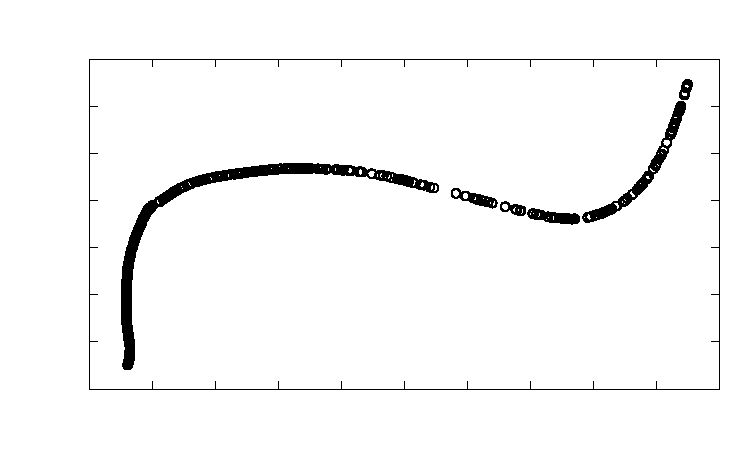
\includegraphics{GRAPH_color_graph1}}%
    \gplfronttext
  \end{picture}%
\endgroup

						}\endgroup
				\caption{A\label{fig:col1}}
			\end{minipage}
			\begin{minipage}[c]{0.5\linewidth}
				\centering
					\begingroup\endlinechar=-1
						\resizebox{\textwidth}{!}{%
							% GNUPLOT: LaTeX picture with Postscript
\begingroup
  \makeatletter
  \providecommand\color[2][]{%
    \GenericError{(gnuplot) \space\space\space\@spaces}{%
      Package color not loaded in conjunction with
      terminal option `colourtext'%
    }{See the gnuplot documentation for explanation.%
    }{Either use 'blacktext' in gnuplot or load the package
      color.sty in LaTeX.}%
    \renewcommand\color[2][]{}%
  }%
  \providecommand\includegraphics[2][]{%
    \GenericError{(gnuplot) \space\space\space\@spaces}{%
      Package graphicx or graphics not loaded%
    }{See the gnuplot documentation for explanation.%
    }{The gnuplot epslatex terminal needs graphicx.sty or graphics.sty.}%
    \renewcommand\includegraphics[2][]{}%
  }%
  \providecommand\rotatebox[2]{#2}%
  \@ifundefined{ifGPcolor}{%
    \newif\ifGPcolor
    \GPcolortrue
  }{}%
  \@ifundefined{ifGPblacktext}{%
    \newif\ifGPblacktext
    \GPblacktexttrue
  }{}%
  % define a \g@addto@macro without @ in the name:
  \let\gplgaddtomacro\g@addto@macro
  % define empty templates for all commands taking text:
  \gdef\gplbacktext{}%
  \gdef\gplfronttext{}%
  \makeatother
  \ifGPblacktext
    % no textcolor at all
    \def\colorrgb#1{}%
    \def\colorgray#1{}%
  \else
    % gray or color?
    \ifGPcolor
      \def\colorrgb#1{\color[rgb]{#1}}%
      \def\colorgray#1{\color[gray]{#1}}%
      \expandafter\def\csname LTw\endcsname{\color{white}}%
      \expandafter\def\csname LTb\endcsname{\color{black}}%
      \expandafter\def\csname LTa\endcsname{\color{black}}%
      \expandafter\def\csname LT0\endcsname{\color[rgb]{1,0,0}}%
      \expandafter\def\csname LT1\endcsname{\color[rgb]{0,1,0}}%
      \expandafter\def\csname LT2\endcsname{\color[rgb]{0,0,1}}%
      \expandafter\def\csname LT3\endcsname{\color[rgb]{1,0,1}}%
      \expandafter\def\csname LT4\endcsname{\color[rgb]{0,1,1}}%
      \expandafter\def\csname LT5\endcsname{\color[rgb]{1,1,0}}%
      \expandafter\def\csname LT6\endcsname{\color[rgb]{0,0,0}}%
      \expandafter\def\csname LT7\endcsname{\color[rgb]{1,0.3,0}}%
      \expandafter\def\csname LT8\endcsname{\color[rgb]{0.5,0.5,0.5}}%
    \else
      % gray
      \def\colorrgb#1{\color{black}}%
      \def\colorgray#1{\color[gray]{#1}}%
      \expandafter\def\csname LTw\endcsname{\color{white}}%
      \expandafter\def\csname LTb\endcsname{\color{black}}%
      \expandafter\def\csname LTa\endcsname{\color{black}}%
      \expandafter\def\csname LT0\endcsname{\color{black}}%
      \expandafter\def\csname LT1\endcsname{\color{black}}%
      \expandafter\def\csname LT2\endcsname{\color{black}}%
      \expandafter\def\csname LT3\endcsname{\color{black}}%
      \expandafter\def\csname LT4\endcsname{\color{black}}%
      \expandafter\def\csname LT5\endcsname{\color{black}}%
      \expandafter\def\csname LT6\endcsname{\color{black}}%
      \expandafter\def\csname LT7\endcsname{\color{black}}%
      \expandafter\def\csname LT8\endcsname{\color{black}}%
    \fi
  \fi
  \setlength{\unitlength}{0.0500bp}%
  \begin{picture}(7200.00,4320.00)%
    \gplgaddtomacro\gplbacktext{%
      \put(849,595){\makebox(0,0)[r]{\strut{} 8}}%
      \put(849,991){\makebox(0,0)[r]{\strut{} 8.5}}%
      \put(849,1387){\makebox(0,0)[r]{\strut{} 9}}%
      \put(849,1782){\makebox(0,0)[r]{\strut{} 9.5}}%
      \put(849,2178){\makebox(0,0)[r]{\strut{} 10}}%
      \put(849,2574){\makebox(0,0)[r]{\strut{} 10.5}}%
      \put(849,2970){\makebox(0,0)[r]{\strut{} 11}}%
      \put(849,3365){\makebox(0,0)[r]{\strut{} 11.5}}%
      \put(849,3761){\makebox(0,0)[r]{\strut{} 12}}%
      \put(951,409){\makebox(0,0){\strut{} 2.5}}%
      \put(1694,409){\makebox(0,0){\strut{} 2.55}}%
      \put(2436,409){\makebox(0,0){\strut{} 2.6}}%
      \put(3179,409){\makebox(0,0){\strut{} 2.65}}%
      \put(3922,409){\makebox(0,0){\strut{} 2.7}}%
      \put(4665,409){\makebox(0,0){\strut{} 2.75}}%
      \put(5407,409){\makebox(0,0){\strut{} 2.8}}%
      \put(6150,409){\makebox(0,0){\strut{} 2.85}}%
      \put(6893,409){\makebox(0,0){\strut{} 2.9}}%
      \csname LTb\endcsname%
      \put(144,2178){\rotatebox{-270}{\makebox(0,0){\strut{}f070w-f090w}}}%
      \csname LTb\endcsname%
      \put(3922,130){\makebox(0,0){\strut{}f090w-f115w}}%
      \put(3922,4040){\makebox(0,0){\strut{}Redshift 7.5--8.5}}%
    }%
    \gplgaddtomacro\gplfronttext{%
    }%
    \gplbacktext
    \put(0,0){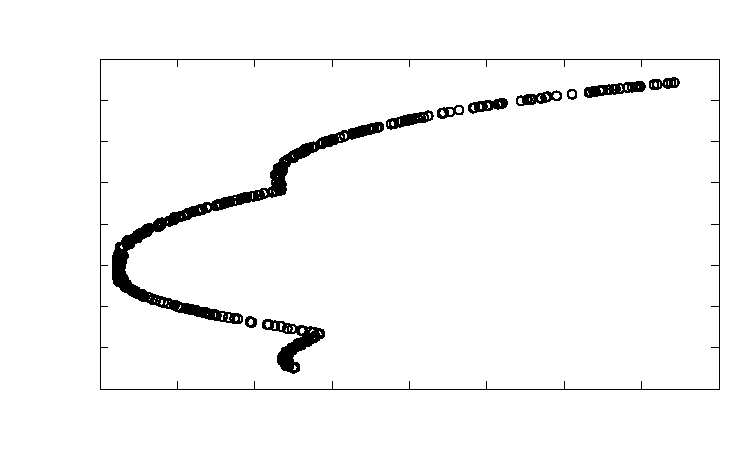
\includegraphics{GRAPH_color_graph2}}%
    \gplfronttext
  \end{picture}%
\endgroup

						}\endgroup
				\caption{B\label{fig:col2}}
			\end{minipage}
			\begin{minipage}[c]{0.5\linewidth}
				\centering
					\begingroup\endlinechar=-1
						\resizebox{\textwidth}{!}{%
							% GNUPLOT: LaTeX picture with Postscript
\begingroup
  \makeatletter
  \providecommand\color[2][]{%
    \GenericError{(gnuplot) \space\space\space\@spaces}{%
      Package color not loaded in conjunction with
      terminal option `colourtext'%
    }{See the gnuplot documentation for explanation.%
    }{Either use 'blacktext' in gnuplot or load the package
      color.sty in LaTeX.}%
    \renewcommand\color[2][]{}%
  }%
  \providecommand\includegraphics[2][]{%
    \GenericError{(gnuplot) \space\space\space\@spaces}{%
      Package graphicx or graphics not loaded%
    }{See the gnuplot documentation for explanation.%
    }{The gnuplot epslatex terminal needs graphicx.sty or graphics.sty.}%
    \renewcommand\includegraphics[2][]{}%
  }%
  \providecommand\rotatebox[2]{#2}%
  \@ifundefined{ifGPcolor}{%
    \newif\ifGPcolor
    \GPcolortrue
  }{}%
  \@ifundefined{ifGPblacktext}{%
    \newif\ifGPblacktext
    \GPblacktexttrue
  }{}%
  % define a \g@addto@macro without @ in the name:
  \let\gplgaddtomacro\g@addto@macro
  % define empty templates for all commands taking text:
  \gdef\gplbacktext{}%
  \gdef\gplfronttext{}%
  \makeatother
  \ifGPblacktext
    % no textcolor at all
    \def\colorrgb#1{}%
    \def\colorgray#1{}%
  \else
    % gray or color?
    \ifGPcolor
      \def\colorrgb#1{\color[rgb]{#1}}%
      \def\colorgray#1{\color[gray]{#1}}%
      \expandafter\def\csname LTw\endcsname{\color{white}}%
      \expandafter\def\csname LTb\endcsname{\color{black}}%
      \expandafter\def\csname LTa\endcsname{\color{black}}%
      \expandafter\def\csname LT0\endcsname{\color[rgb]{1,0,0}}%
      \expandafter\def\csname LT1\endcsname{\color[rgb]{0,1,0}}%
      \expandafter\def\csname LT2\endcsname{\color[rgb]{0,0,1}}%
      \expandafter\def\csname LT3\endcsname{\color[rgb]{1,0,1}}%
      \expandafter\def\csname LT4\endcsname{\color[rgb]{0,1,1}}%
      \expandafter\def\csname LT5\endcsname{\color[rgb]{1,1,0}}%
      \expandafter\def\csname LT6\endcsname{\color[rgb]{0,0,0}}%
      \expandafter\def\csname LT7\endcsname{\color[rgb]{1,0.3,0}}%
      \expandafter\def\csname LT8\endcsname{\color[rgb]{0.5,0.5,0.5}}%
    \else
      % gray
      \def\colorrgb#1{\color{black}}%
      \def\colorgray#1{\color[gray]{#1}}%
      \expandafter\def\csname LTw\endcsname{\color{white}}%
      \expandafter\def\csname LTb\endcsname{\color{black}}%
      \expandafter\def\csname LTa\endcsname{\color{black}}%
      \expandafter\def\csname LT0\endcsname{\color{black}}%
      \expandafter\def\csname LT1\endcsname{\color{black}}%
      \expandafter\def\csname LT2\endcsname{\color{black}}%
      \expandafter\def\csname LT3\endcsname{\color{black}}%
      \expandafter\def\csname LT4\endcsname{\color{black}}%
      \expandafter\def\csname LT5\endcsname{\color{black}}%
      \expandafter\def\csname LT6\endcsname{\color{black}}%
      \expandafter\def\csname LT7\endcsname{\color{black}}%
      \expandafter\def\csname LT8\endcsname{\color{black}}%
    \fi
  \fi
  \setlength{\unitlength}{0.0500bp}%
  \begin{picture}(7200.00,4320.00)%
    \gplgaddtomacro\gplbacktext{%
      \put(849,595){\makebox(0,0)[r]{\strut{} 11}}%
      \put(849,912){\makebox(0,0)[r]{\strut{} 11.5}}%
      \put(849,1228){\makebox(0,0)[r]{\strut{} 12}}%
      \put(849,1545){\makebox(0,0)[r]{\strut{} 12.5}}%
      \put(849,1861){\makebox(0,0)[r]{\strut{} 13}}%
      \put(849,2178){\makebox(0,0)[r]{\strut{} 13.5}}%
      \put(849,2495){\makebox(0,0)[r]{\strut{} 14}}%
      \put(849,2811){\makebox(0,0)[r]{\strut{} 14.5}}%
      \put(849,3128){\makebox(0,0)[r]{\strut{} 15}}%
      \put(849,3444){\makebox(0,0)[r]{\strut{} 15.5}}%
      \put(849,3761){\makebox(0,0)[r]{\strut{} 16}}%
      \put(951,409){\makebox(0,0){\strut{} 1.5}}%
      \put(1694,409){\makebox(0,0){\strut{} 2}}%
      \put(2437,409){\makebox(0,0){\strut{} 2.5}}%
      \put(3179,409){\makebox(0,0){\strut{} 3}}%
      \put(3922,409){\makebox(0,0){\strut{} 3.5}}%
      \put(4665,409){\makebox(0,0){\strut{} 4}}%
      \put(5408,409){\makebox(0,0){\strut{} 4.5}}%
      \put(6150,409){\makebox(0,0){\strut{} 5}}%
      \put(6893,409){\makebox(0,0){\strut{} 5.5}}%
      \csname LTb\endcsname%
      \put(144,2178){\rotatebox{-270}{\makebox(0,0){\strut{}Y-J}}}%
      \csname LTb\endcsname%
      \put(3922,130){\makebox(0,0){\strut{}J-H}}%
      \put(3922,4040){\makebox(0,0){\strut{}Redshift 8.5--10.1}}%
    }%
    \gplgaddtomacro\gplfronttext{%
    }%
    \gplbacktext
    \put(0,0){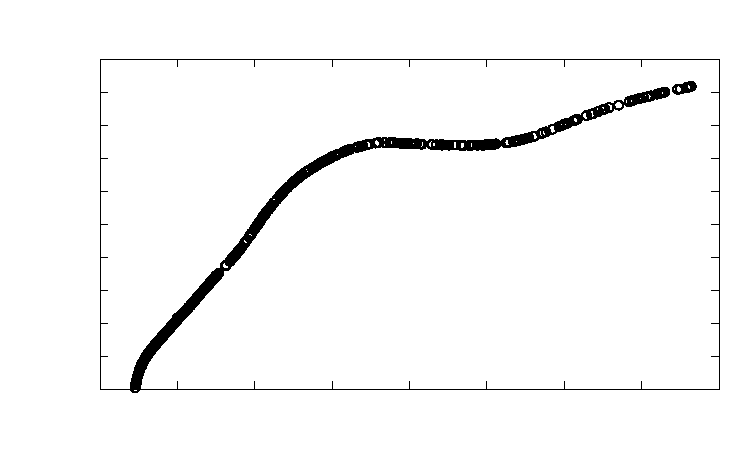
\includegraphics{GRAPH_color_graph3}}%
    \gplfronttext
  \end{picture}%
\endgroup

						}\endgroup
				\caption{C\label{fig:col3}}
			\end{minipage}
			\begin{minipage}[c]{0.5\linewidth}
				\centering
					\begingroup\endlinechar=-1
						\resizebox{\textwidth}{!}{%
							% GNUPLOT: LaTeX picture with Postscript
\begingroup
  \makeatletter
  \providecommand\color[2][]{%
    \GenericError{(gnuplot) \space\space\space\@spaces}{%
      Package color not loaded in conjunction with
      terminal option `colourtext'%
    }{See the gnuplot documentation for explanation.%
    }{Either use 'blacktext' in gnuplot or load the package
      color.sty in LaTeX.}%
    \renewcommand\color[2][]{}%
  }%
  \providecommand\includegraphics[2][]{%
    \GenericError{(gnuplot) \space\space\space\@spaces}{%
      Package graphicx or graphics not loaded%
    }{See the gnuplot documentation for explanation.%
    }{The gnuplot epslatex terminal needs graphicx.sty or graphics.sty.}%
    \renewcommand\includegraphics[2][]{}%
  }%
  \providecommand\rotatebox[2]{#2}%
  \@ifundefined{ifGPcolor}{%
    \newif\ifGPcolor
    \GPcolortrue
  }{}%
  \@ifundefined{ifGPblacktext}{%
    \newif\ifGPblacktext
    \GPblacktexttrue
  }{}%
  % define a \g@addto@macro without @ in the name:
  \let\gplgaddtomacro\g@addto@macro
  % define empty templates for all commands taking text:
  \gdef\gplbacktext{}%
  \gdef\gplfronttext{}%
  \makeatother
  \ifGPblacktext
    % no textcolor at all
    \def\colorrgb#1{}%
    \def\colorgray#1{}%
  \else
    % gray or color?
    \ifGPcolor
      \def\colorrgb#1{\color[rgb]{#1}}%
      \def\colorgray#1{\color[gray]{#1}}%
      \expandafter\def\csname LTw\endcsname{\color{white}}%
      \expandafter\def\csname LTb\endcsname{\color{black}}%
      \expandafter\def\csname LTa\endcsname{\color{black}}%
      \expandafter\def\csname LT0\endcsname{\color[rgb]{1,0,0}}%
      \expandafter\def\csname LT1\endcsname{\color[rgb]{0,1,0}}%
      \expandafter\def\csname LT2\endcsname{\color[rgb]{0,0,1}}%
      \expandafter\def\csname LT3\endcsname{\color[rgb]{1,0,1}}%
      \expandafter\def\csname LT4\endcsname{\color[rgb]{0,1,1}}%
      \expandafter\def\csname LT5\endcsname{\color[rgb]{1,1,0}}%
      \expandafter\def\csname LT6\endcsname{\color[rgb]{0,0,0}}%
      \expandafter\def\csname LT7\endcsname{\color[rgb]{1,0.3,0}}%
      \expandafter\def\csname LT8\endcsname{\color[rgb]{0.5,0.5,0.5}}%
    \else
      % gray
      \def\colorrgb#1{\color{black}}%
      \def\colorgray#1{\color[gray]{#1}}%
      \expandafter\def\csname LTw\endcsname{\color{white}}%
      \expandafter\def\csname LTb\endcsname{\color{black}}%
      \expandafter\def\csname LTa\endcsname{\color{black}}%
      \expandafter\def\csname LT0\endcsname{\color{black}}%
      \expandafter\def\csname LT1\endcsname{\color{black}}%
      \expandafter\def\csname LT2\endcsname{\color{black}}%
      \expandafter\def\csname LT3\endcsname{\color{black}}%
      \expandafter\def\csname LT4\endcsname{\color{black}}%
      \expandafter\def\csname LT5\endcsname{\color{black}}%
      \expandafter\def\csname LT6\endcsname{\color{black}}%
      \expandafter\def\csname LT7\endcsname{\color{black}}%
      \expandafter\def\csname LT8\endcsname{\color{black}}%
    \fi
  \fi
  \setlength{\unitlength}{0.0500bp}%
  \begin{picture}(7200.00,4320.00)%
    \gplgaddtomacro\gplbacktext{%
      \put(645,595){\makebox(0,0)[r]{\strut{} 10}}%
      \put(645,947){\makebox(0,0)[r]{\strut{} 15}}%
      \put(645,1299){\makebox(0,0)[r]{\strut{} 20}}%
      \put(645,1650){\makebox(0,0)[r]{\strut{} 25}}%
      \put(645,2002){\makebox(0,0)[r]{\strut{} 30}}%
      \put(645,2354){\makebox(0,0)[r]{\strut{} 35}}%
      \put(645,2706){\makebox(0,0)[r]{\strut{} 40}}%
      \put(645,3057){\makebox(0,0)[r]{\strut{} 45}}%
      \put(645,3409){\makebox(0,0)[r]{\strut{} 50}}%
      \put(645,3761){\makebox(0,0)[r]{\strut{} 55}}%
      \put(747,409){\makebox(0,0){\strut{} 0}}%
      \put(1515,409){\makebox(0,0){\strut{} 2}}%
      \put(2284,409){\makebox(0,0){\strut{} 4}}%
      \put(3052,409){\makebox(0,0){\strut{} 6}}%
      \put(3820,409){\makebox(0,0){\strut{} 8}}%
      \put(4588,409){\makebox(0,0){\strut{} 10}}%
      \put(5357,409){\makebox(0,0){\strut{} 12}}%
      \put(6125,409){\makebox(0,0){\strut{} 14}}%
      \put(6893,409){\makebox(0,0){\strut{} 16}}%
      \csname LTb\endcsname%
      \put(144,2178){\rotatebox{-270}{\makebox(0,0){\strut{}f150w-f200w}}}%
      \csname LTb\endcsname%
      \put(3820,130){\makebox(0,0){\strut{}f115w-f150w}}%
      \put(3820,4040){\makebox(0,0){\strut{}Redshift 10--14}}%
    }%
    \gplgaddtomacro\gplfronttext{%
    }%
    \gplbacktext
    \put(0,0){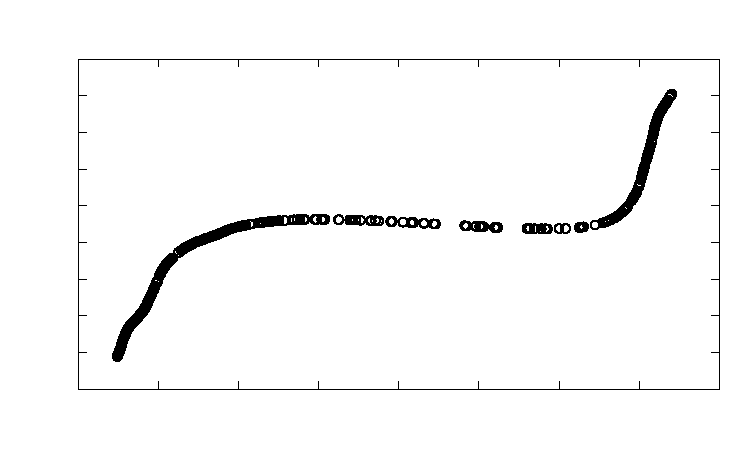
\includegraphics{GRAPH_color_graph4}}%
    \gplfronttext
  \end{picture}%
\endgroup

						}\endgroup
				\caption{D\label{fig:col4}}
			\end{minipage}
			\caption{Graphs showing the colour-colour regions for \\
			(A) z=6-7.5. The colour window was defined as $f070w-f090w{\ge}3.257$ and $f090w-f115w{\le}8.242$,\\
			(B) z=7.5-8.5. The colour window was defined as $f090w-f115w{\ge}8.251$ and $f115w-f150w{\le}2.869$, \\
			(C) z=8.54-10.1. The colour window was defined as $Y-J{\ge}11.019$ and $J-H{\le}5.298$, \\
			(D) z=10-14. The colour window was defined as $f115w-f150w{\ge}14.439$ and $f150w-f200w{\le}14.815$}
		\end{figure}

		% \begin{figure}[!htbp]
		% 	\centering
		% 		\begingroup\endlinechar=-1
		% 			\resizebox{0.7\textwidth}{!}{%
		% 				% GNUPLOT: LaTeX picture with Postscript
\begingroup
  \makeatletter
  \providecommand\color[2][]{%
    \GenericError{(gnuplot) \space\space\space\@spaces}{%
      Package color not loaded in conjunction with
      terminal option `colourtext'%
    }{See the gnuplot documentation for explanation.%
    }{Either use 'blacktext' in gnuplot or load the package
      color.sty in LaTeX.}%
    \renewcommand\color[2][]{}%
  }%
  \providecommand\includegraphics[2][]{%
    \GenericError{(gnuplot) \space\space\space\@spaces}{%
      Package graphicx or graphics not loaded%
    }{See the gnuplot documentation for explanation.%
    }{The gnuplot epslatex terminal needs graphicx.sty or graphics.sty.}%
    \renewcommand\includegraphics[2][]{}%
  }%
  \providecommand\rotatebox[2]{#2}%
  \@ifundefined{ifGPcolor}{%
    \newif\ifGPcolor
    \GPcolortrue
  }{}%
  \@ifundefined{ifGPblacktext}{%
    \newif\ifGPblacktext
    \GPblacktexttrue
  }{}%
  % define a \g@addto@macro without @ in the name:
  \let\gplgaddtomacro\g@addto@macro
  % define empty templates for all commands taking text:
  \gdef\gplbacktext{}%
  \gdef\gplfronttext{}%
  \makeatother
  \ifGPblacktext
    % no textcolor at all
    \def\colorrgb#1{}%
    \def\colorgray#1{}%
  \else
    % gray or color?
    \ifGPcolor
      \def\colorrgb#1{\color[rgb]{#1}}%
      \def\colorgray#1{\color[gray]{#1}}%
      \expandafter\def\csname LTw\endcsname{\color{white}}%
      \expandafter\def\csname LTb\endcsname{\color{black}}%
      \expandafter\def\csname LTa\endcsname{\color{black}}%
      \expandafter\def\csname LT0\endcsname{\color[rgb]{1,0,0}}%
      \expandafter\def\csname LT1\endcsname{\color[rgb]{0,1,0}}%
      \expandafter\def\csname LT2\endcsname{\color[rgb]{0,0,1}}%
      \expandafter\def\csname LT3\endcsname{\color[rgb]{1,0,1}}%
      \expandafter\def\csname LT4\endcsname{\color[rgb]{0,1,1}}%
      \expandafter\def\csname LT5\endcsname{\color[rgb]{1,1,0}}%
      \expandafter\def\csname LT6\endcsname{\color[rgb]{0,0,0}}%
      \expandafter\def\csname LT7\endcsname{\color[rgb]{1,0.3,0}}%
      \expandafter\def\csname LT8\endcsname{\color[rgb]{0.5,0.5,0.5}}%
    \else
      % gray
      \def\colorrgb#1{\color{black}}%
      \def\colorgray#1{\color[gray]{#1}}%
      \expandafter\def\csname LTw\endcsname{\color{white}}%
      \expandafter\def\csname LTb\endcsname{\color{black}}%
      \expandafter\def\csname LTa\endcsname{\color{black}}%
      \expandafter\def\csname LT0\endcsname{\color{black}}%
      \expandafter\def\csname LT1\endcsname{\color{black}}%
      \expandafter\def\csname LT2\endcsname{\color{black}}%
      \expandafter\def\csname LT3\endcsname{\color{black}}%
      \expandafter\def\csname LT4\endcsname{\color{black}}%
      \expandafter\def\csname LT5\endcsname{\color{black}}%
      \expandafter\def\csname LT6\endcsname{\color{black}}%
      \expandafter\def\csname LT7\endcsname{\color{black}}%
      \expandafter\def\csname LT8\endcsname{\color{black}}%
    \fi
  \fi
  \setlength{\unitlength}{0.0500bp}%
  \begin{picture}(7200.00,4320.00)%
    \gplgaddtomacro\gplbacktext{%
      \put(747,595){\makebox(0,0)[r]{\strut{} 3}}%
      \put(747,1047){\makebox(0,0)[r]{\strut{} 3.5}}%
      \put(747,1500){\makebox(0,0)[r]{\strut{} 4}}%
      \put(747,1952){\makebox(0,0)[r]{\strut{} 4.5}}%
      \put(747,2404){\makebox(0,0)[r]{\strut{} 5}}%
      \put(747,2856){\makebox(0,0)[r]{\strut{} 5.5}}%
      \put(747,3309){\makebox(0,0)[r]{\strut{} 6}}%
      \put(747,3761){\makebox(0,0)[r]{\strut{} 6.5}}%
      \put(849,409){\makebox(0,0){\strut{} 3.5}}%
      \put(1453,409){\makebox(0,0){\strut{} 4}}%
      \put(2058,409){\makebox(0,0){\strut{} 4.5}}%
      \put(2662,409){\makebox(0,0){\strut{} 5}}%
      \put(3267,409){\makebox(0,0){\strut{} 5.5}}%
      \put(3871,409){\makebox(0,0){\strut{} 6}}%
      \put(4475,409){\makebox(0,0){\strut{} 6.5}}%
      \put(5080,409){\makebox(0,0){\strut{} 7}}%
      \put(5684,409){\makebox(0,0){\strut{} 7.5}}%
      \put(6289,409){\makebox(0,0){\strut{} 8}}%
      \put(6893,409){\makebox(0,0){\strut{} 8.5}}%
      \csname LTb\endcsname%
      \put(144,2178){\rotatebox{-270}{\makebox(0,0){\strut{}f070w-f090w}}}%
      \csname LTb\endcsname%
      \put(3871,130){\makebox(0,0){\strut{}f090w-f115w}}%
      \put(3871,4040){\makebox(0,0){\strut{}Redshift 6--7.5}}%
    }%
    \gplgaddtomacro\gplfronttext{%
    }%
    \gplbacktext
    \put(0,0){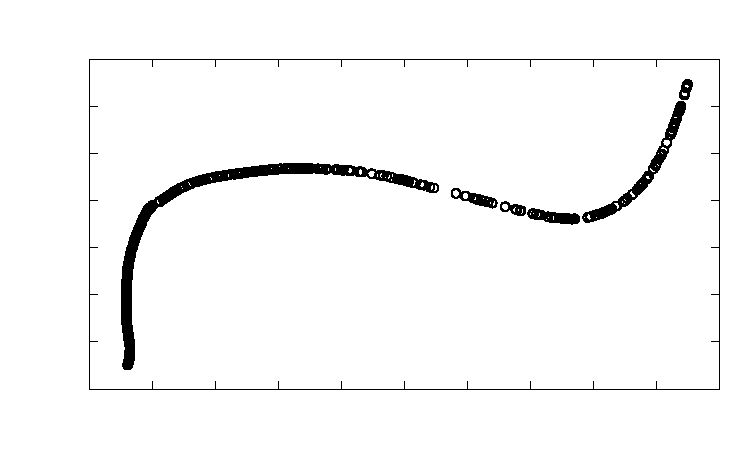
\includegraphics{GRAPH_color_graph1}}%
    \gplfronttext
  \end{picture}%
\endgroup

		% 			}\endgroup
		% 	\caption{Graph showing the colour-colour region for z=6-7.5. The colour window was defined as $f070w-f090w{\ge}3.257$ and $f090w-f115w{\le}8.242$.\label{fig:col1}}
		% \end{figure}
		% \begin{figure}[!htbp]
		% 	\centering
		% 		\begingroup\endlinechar=-1
		% 			\resizebox{0.7\textwidth}{!}{%
		% 				% GNUPLOT: LaTeX picture with Postscript
\begingroup
  \makeatletter
  \providecommand\color[2][]{%
    \GenericError{(gnuplot) \space\space\space\@spaces}{%
      Package color not loaded in conjunction with
      terminal option `colourtext'%
    }{See the gnuplot documentation for explanation.%
    }{Either use 'blacktext' in gnuplot or load the package
      color.sty in LaTeX.}%
    \renewcommand\color[2][]{}%
  }%
  \providecommand\includegraphics[2][]{%
    \GenericError{(gnuplot) \space\space\space\@spaces}{%
      Package graphicx or graphics not loaded%
    }{See the gnuplot documentation for explanation.%
    }{The gnuplot epslatex terminal needs graphicx.sty or graphics.sty.}%
    \renewcommand\includegraphics[2][]{}%
  }%
  \providecommand\rotatebox[2]{#2}%
  \@ifundefined{ifGPcolor}{%
    \newif\ifGPcolor
    \GPcolortrue
  }{}%
  \@ifundefined{ifGPblacktext}{%
    \newif\ifGPblacktext
    \GPblacktexttrue
  }{}%
  % define a \g@addto@macro without @ in the name:
  \let\gplgaddtomacro\g@addto@macro
  % define empty templates for all commands taking text:
  \gdef\gplbacktext{}%
  \gdef\gplfronttext{}%
  \makeatother
  \ifGPblacktext
    % no textcolor at all
    \def\colorrgb#1{}%
    \def\colorgray#1{}%
  \else
    % gray or color?
    \ifGPcolor
      \def\colorrgb#1{\color[rgb]{#1}}%
      \def\colorgray#1{\color[gray]{#1}}%
      \expandafter\def\csname LTw\endcsname{\color{white}}%
      \expandafter\def\csname LTb\endcsname{\color{black}}%
      \expandafter\def\csname LTa\endcsname{\color{black}}%
      \expandafter\def\csname LT0\endcsname{\color[rgb]{1,0,0}}%
      \expandafter\def\csname LT1\endcsname{\color[rgb]{0,1,0}}%
      \expandafter\def\csname LT2\endcsname{\color[rgb]{0,0,1}}%
      \expandafter\def\csname LT3\endcsname{\color[rgb]{1,0,1}}%
      \expandafter\def\csname LT4\endcsname{\color[rgb]{0,1,1}}%
      \expandafter\def\csname LT5\endcsname{\color[rgb]{1,1,0}}%
      \expandafter\def\csname LT6\endcsname{\color[rgb]{0,0,0}}%
      \expandafter\def\csname LT7\endcsname{\color[rgb]{1,0.3,0}}%
      \expandafter\def\csname LT8\endcsname{\color[rgb]{0.5,0.5,0.5}}%
    \else
      % gray
      \def\colorrgb#1{\color{black}}%
      \def\colorgray#1{\color[gray]{#1}}%
      \expandafter\def\csname LTw\endcsname{\color{white}}%
      \expandafter\def\csname LTb\endcsname{\color{black}}%
      \expandafter\def\csname LTa\endcsname{\color{black}}%
      \expandafter\def\csname LT0\endcsname{\color{black}}%
      \expandafter\def\csname LT1\endcsname{\color{black}}%
      \expandafter\def\csname LT2\endcsname{\color{black}}%
      \expandafter\def\csname LT3\endcsname{\color{black}}%
      \expandafter\def\csname LT4\endcsname{\color{black}}%
      \expandafter\def\csname LT5\endcsname{\color{black}}%
      \expandafter\def\csname LT6\endcsname{\color{black}}%
      \expandafter\def\csname LT7\endcsname{\color{black}}%
      \expandafter\def\csname LT8\endcsname{\color{black}}%
    \fi
  \fi
  \setlength{\unitlength}{0.0500bp}%
  \begin{picture}(7200.00,4320.00)%
    \gplgaddtomacro\gplbacktext{%
      \put(849,595){\makebox(0,0)[r]{\strut{} 8}}%
      \put(849,991){\makebox(0,0)[r]{\strut{} 8.5}}%
      \put(849,1387){\makebox(0,0)[r]{\strut{} 9}}%
      \put(849,1782){\makebox(0,0)[r]{\strut{} 9.5}}%
      \put(849,2178){\makebox(0,0)[r]{\strut{} 10}}%
      \put(849,2574){\makebox(0,0)[r]{\strut{} 10.5}}%
      \put(849,2970){\makebox(0,0)[r]{\strut{} 11}}%
      \put(849,3365){\makebox(0,0)[r]{\strut{} 11.5}}%
      \put(849,3761){\makebox(0,0)[r]{\strut{} 12}}%
      \put(951,409){\makebox(0,0){\strut{} 2.5}}%
      \put(1694,409){\makebox(0,0){\strut{} 2.55}}%
      \put(2436,409){\makebox(0,0){\strut{} 2.6}}%
      \put(3179,409){\makebox(0,0){\strut{} 2.65}}%
      \put(3922,409){\makebox(0,0){\strut{} 2.7}}%
      \put(4665,409){\makebox(0,0){\strut{} 2.75}}%
      \put(5407,409){\makebox(0,0){\strut{} 2.8}}%
      \put(6150,409){\makebox(0,0){\strut{} 2.85}}%
      \put(6893,409){\makebox(0,0){\strut{} 2.9}}%
      \csname LTb\endcsname%
      \put(144,2178){\rotatebox{-270}{\makebox(0,0){\strut{}f070w-f090w}}}%
      \csname LTb\endcsname%
      \put(3922,130){\makebox(0,0){\strut{}f090w-f115w}}%
      \put(3922,4040){\makebox(0,0){\strut{}Redshift 7.5--8.5}}%
    }%
    \gplgaddtomacro\gplfronttext{%
    }%
    \gplbacktext
    \put(0,0){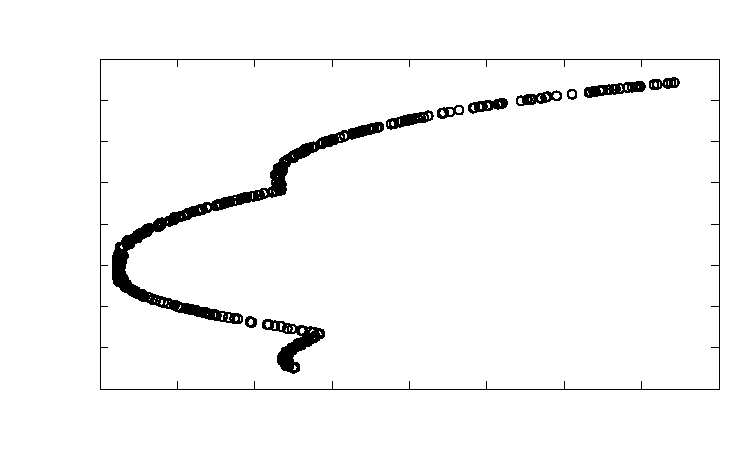
\includegraphics{GRAPH_color_graph2}}%
    \gplfronttext
  \end{picture}%
\endgroup

		% 			}\endgroup
		% 	\caption{Graph showing the colour-colour region for z=7.5-8.5. The colour window was defined as $f090w-f115w{\ge}8.251$ and $f115w-f150w{\le}2.869$\label{fig:col2}}
		% \end{figure}
		% \begin{figure}[!htbp]
		% 	\centering
		% 		\begingroup\endlinechar=-1
		% 			\resizebox{0.7\textwidth}{!}{%
		% 				% GNUPLOT: LaTeX picture with Postscript
\begingroup
  \makeatletter
  \providecommand\color[2][]{%
    \GenericError{(gnuplot) \space\space\space\@spaces}{%
      Package color not loaded in conjunction with
      terminal option `colourtext'%
    }{See the gnuplot documentation for explanation.%
    }{Either use 'blacktext' in gnuplot or load the package
      color.sty in LaTeX.}%
    \renewcommand\color[2][]{}%
  }%
  \providecommand\includegraphics[2][]{%
    \GenericError{(gnuplot) \space\space\space\@spaces}{%
      Package graphicx or graphics not loaded%
    }{See the gnuplot documentation for explanation.%
    }{The gnuplot epslatex terminal needs graphicx.sty or graphics.sty.}%
    \renewcommand\includegraphics[2][]{}%
  }%
  \providecommand\rotatebox[2]{#2}%
  \@ifundefined{ifGPcolor}{%
    \newif\ifGPcolor
    \GPcolortrue
  }{}%
  \@ifundefined{ifGPblacktext}{%
    \newif\ifGPblacktext
    \GPblacktexttrue
  }{}%
  % define a \g@addto@macro without @ in the name:
  \let\gplgaddtomacro\g@addto@macro
  % define empty templates for all commands taking text:
  \gdef\gplbacktext{}%
  \gdef\gplfronttext{}%
  \makeatother
  \ifGPblacktext
    % no textcolor at all
    \def\colorrgb#1{}%
    \def\colorgray#1{}%
  \else
    % gray or color?
    \ifGPcolor
      \def\colorrgb#1{\color[rgb]{#1}}%
      \def\colorgray#1{\color[gray]{#1}}%
      \expandafter\def\csname LTw\endcsname{\color{white}}%
      \expandafter\def\csname LTb\endcsname{\color{black}}%
      \expandafter\def\csname LTa\endcsname{\color{black}}%
      \expandafter\def\csname LT0\endcsname{\color[rgb]{1,0,0}}%
      \expandafter\def\csname LT1\endcsname{\color[rgb]{0,1,0}}%
      \expandafter\def\csname LT2\endcsname{\color[rgb]{0,0,1}}%
      \expandafter\def\csname LT3\endcsname{\color[rgb]{1,0,1}}%
      \expandafter\def\csname LT4\endcsname{\color[rgb]{0,1,1}}%
      \expandafter\def\csname LT5\endcsname{\color[rgb]{1,1,0}}%
      \expandafter\def\csname LT6\endcsname{\color[rgb]{0,0,0}}%
      \expandafter\def\csname LT7\endcsname{\color[rgb]{1,0.3,0}}%
      \expandafter\def\csname LT8\endcsname{\color[rgb]{0.5,0.5,0.5}}%
    \else
      % gray
      \def\colorrgb#1{\color{black}}%
      \def\colorgray#1{\color[gray]{#1}}%
      \expandafter\def\csname LTw\endcsname{\color{white}}%
      \expandafter\def\csname LTb\endcsname{\color{black}}%
      \expandafter\def\csname LTa\endcsname{\color{black}}%
      \expandafter\def\csname LT0\endcsname{\color{black}}%
      \expandafter\def\csname LT1\endcsname{\color{black}}%
      \expandafter\def\csname LT2\endcsname{\color{black}}%
      \expandafter\def\csname LT3\endcsname{\color{black}}%
      \expandafter\def\csname LT4\endcsname{\color{black}}%
      \expandafter\def\csname LT5\endcsname{\color{black}}%
      \expandafter\def\csname LT6\endcsname{\color{black}}%
      \expandafter\def\csname LT7\endcsname{\color{black}}%
      \expandafter\def\csname LT8\endcsname{\color{black}}%
    \fi
  \fi
  \setlength{\unitlength}{0.0500bp}%
  \begin{picture}(7200.00,4320.00)%
    \gplgaddtomacro\gplbacktext{%
      \put(849,595){\makebox(0,0)[r]{\strut{} 11}}%
      \put(849,912){\makebox(0,0)[r]{\strut{} 11.5}}%
      \put(849,1228){\makebox(0,0)[r]{\strut{} 12}}%
      \put(849,1545){\makebox(0,0)[r]{\strut{} 12.5}}%
      \put(849,1861){\makebox(0,0)[r]{\strut{} 13}}%
      \put(849,2178){\makebox(0,0)[r]{\strut{} 13.5}}%
      \put(849,2495){\makebox(0,0)[r]{\strut{} 14}}%
      \put(849,2811){\makebox(0,0)[r]{\strut{} 14.5}}%
      \put(849,3128){\makebox(0,0)[r]{\strut{} 15}}%
      \put(849,3444){\makebox(0,0)[r]{\strut{} 15.5}}%
      \put(849,3761){\makebox(0,0)[r]{\strut{} 16}}%
      \put(951,409){\makebox(0,0){\strut{} 1.5}}%
      \put(1694,409){\makebox(0,0){\strut{} 2}}%
      \put(2437,409){\makebox(0,0){\strut{} 2.5}}%
      \put(3179,409){\makebox(0,0){\strut{} 3}}%
      \put(3922,409){\makebox(0,0){\strut{} 3.5}}%
      \put(4665,409){\makebox(0,0){\strut{} 4}}%
      \put(5408,409){\makebox(0,0){\strut{} 4.5}}%
      \put(6150,409){\makebox(0,0){\strut{} 5}}%
      \put(6893,409){\makebox(0,0){\strut{} 5.5}}%
      \csname LTb\endcsname%
      \put(144,2178){\rotatebox{-270}{\makebox(0,0){\strut{}Y-J}}}%
      \csname LTb\endcsname%
      \put(3922,130){\makebox(0,0){\strut{}J-H}}%
      \put(3922,4040){\makebox(0,0){\strut{}Redshift 8.5--10.1}}%
    }%
    \gplgaddtomacro\gplfronttext{%
    }%
    \gplbacktext
    \put(0,0){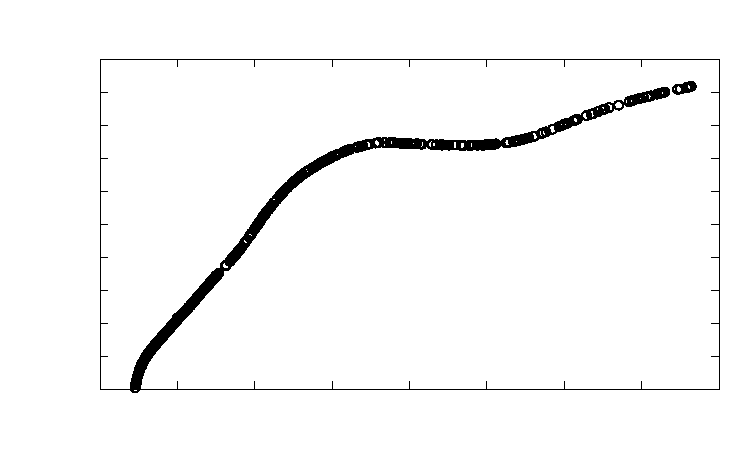
\includegraphics{GRAPH_color_graph3}}%
    \gplfronttext
  \end{picture}%
\endgroup

		% 			}\endgroup
		% 	\caption{Graph showing the colour-colour region for z=8.54-10.1. The colour window was defined as $Y-J{\ge}11.019$ and $J-H{\le}5.298$\label{fig:col3}}
		% \end{figure}
		% \begin{figure}[!htbp]
		% 	\centering
		% 		\begingroup\endlinechar=-1
		% 			\resizebox{0.7\textwidth}{!}{%
		% 				% GNUPLOT: LaTeX picture with Postscript
\begingroup
  \makeatletter
  \providecommand\color[2][]{%
    \GenericError{(gnuplot) \space\space\space\@spaces}{%
      Package color not loaded in conjunction with
      terminal option `colourtext'%
    }{See the gnuplot documentation for explanation.%
    }{Either use 'blacktext' in gnuplot or load the package
      color.sty in LaTeX.}%
    \renewcommand\color[2][]{}%
  }%
  \providecommand\includegraphics[2][]{%
    \GenericError{(gnuplot) \space\space\space\@spaces}{%
      Package graphicx or graphics not loaded%
    }{See the gnuplot documentation for explanation.%
    }{The gnuplot epslatex terminal needs graphicx.sty or graphics.sty.}%
    \renewcommand\includegraphics[2][]{}%
  }%
  \providecommand\rotatebox[2]{#2}%
  \@ifundefined{ifGPcolor}{%
    \newif\ifGPcolor
    \GPcolortrue
  }{}%
  \@ifundefined{ifGPblacktext}{%
    \newif\ifGPblacktext
    \GPblacktexttrue
  }{}%
  % define a \g@addto@macro without @ in the name:
  \let\gplgaddtomacro\g@addto@macro
  % define empty templates for all commands taking text:
  \gdef\gplbacktext{}%
  \gdef\gplfronttext{}%
  \makeatother
  \ifGPblacktext
    % no textcolor at all
    \def\colorrgb#1{}%
    \def\colorgray#1{}%
  \else
    % gray or color?
    \ifGPcolor
      \def\colorrgb#1{\color[rgb]{#1}}%
      \def\colorgray#1{\color[gray]{#1}}%
      \expandafter\def\csname LTw\endcsname{\color{white}}%
      \expandafter\def\csname LTb\endcsname{\color{black}}%
      \expandafter\def\csname LTa\endcsname{\color{black}}%
      \expandafter\def\csname LT0\endcsname{\color[rgb]{1,0,0}}%
      \expandafter\def\csname LT1\endcsname{\color[rgb]{0,1,0}}%
      \expandafter\def\csname LT2\endcsname{\color[rgb]{0,0,1}}%
      \expandafter\def\csname LT3\endcsname{\color[rgb]{1,0,1}}%
      \expandafter\def\csname LT4\endcsname{\color[rgb]{0,1,1}}%
      \expandafter\def\csname LT5\endcsname{\color[rgb]{1,1,0}}%
      \expandafter\def\csname LT6\endcsname{\color[rgb]{0,0,0}}%
      \expandafter\def\csname LT7\endcsname{\color[rgb]{1,0.3,0}}%
      \expandafter\def\csname LT8\endcsname{\color[rgb]{0.5,0.5,0.5}}%
    \else
      % gray
      \def\colorrgb#1{\color{black}}%
      \def\colorgray#1{\color[gray]{#1}}%
      \expandafter\def\csname LTw\endcsname{\color{white}}%
      \expandafter\def\csname LTb\endcsname{\color{black}}%
      \expandafter\def\csname LTa\endcsname{\color{black}}%
      \expandafter\def\csname LT0\endcsname{\color{black}}%
      \expandafter\def\csname LT1\endcsname{\color{black}}%
      \expandafter\def\csname LT2\endcsname{\color{black}}%
      \expandafter\def\csname LT3\endcsname{\color{black}}%
      \expandafter\def\csname LT4\endcsname{\color{black}}%
      \expandafter\def\csname LT5\endcsname{\color{black}}%
      \expandafter\def\csname LT6\endcsname{\color{black}}%
      \expandafter\def\csname LT7\endcsname{\color{black}}%
      \expandafter\def\csname LT8\endcsname{\color{black}}%
    \fi
  \fi
  \setlength{\unitlength}{0.0500bp}%
  \begin{picture}(7200.00,4320.00)%
    \gplgaddtomacro\gplbacktext{%
      \put(645,595){\makebox(0,0)[r]{\strut{} 10}}%
      \put(645,947){\makebox(0,0)[r]{\strut{} 15}}%
      \put(645,1299){\makebox(0,0)[r]{\strut{} 20}}%
      \put(645,1650){\makebox(0,0)[r]{\strut{} 25}}%
      \put(645,2002){\makebox(0,0)[r]{\strut{} 30}}%
      \put(645,2354){\makebox(0,0)[r]{\strut{} 35}}%
      \put(645,2706){\makebox(0,0)[r]{\strut{} 40}}%
      \put(645,3057){\makebox(0,0)[r]{\strut{} 45}}%
      \put(645,3409){\makebox(0,0)[r]{\strut{} 50}}%
      \put(645,3761){\makebox(0,0)[r]{\strut{} 55}}%
      \put(747,409){\makebox(0,0){\strut{} 0}}%
      \put(1515,409){\makebox(0,0){\strut{} 2}}%
      \put(2284,409){\makebox(0,0){\strut{} 4}}%
      \put(3052,409){\makebox(0,0){\strut{} 6}}%
      \put(3820,409){\makebox(0,0){\strut{} 8}}%
      \put(4588,409){\makebox(0,0){\strut{} 10}}%
      \put(5357,409){\makebox(0,0){\strut{} 12}}%
      \put(6125,409){\makebox(0,0){\strut{} 14}}%
      \put(6893,409){\makebox(0,0){\strut{} 16}}%
      \csname LTb\endcsname%
      \put(144,2178){\rotatebox{-270}{\makebox(0,0){\strut{}f150w-f200w}}}%
      \csname LTb\endcsname%
      \put(3820,130){\makebox(0,0){\strut{}f115w-f150w}}%
      \put(3820,4040){\makebox(0,0){\strut{}Redshift 10--14}}%
    }%
    \gplgaddtomacro\gplfronttext{%
    }%
    \gplbacktext
    \put(0,0){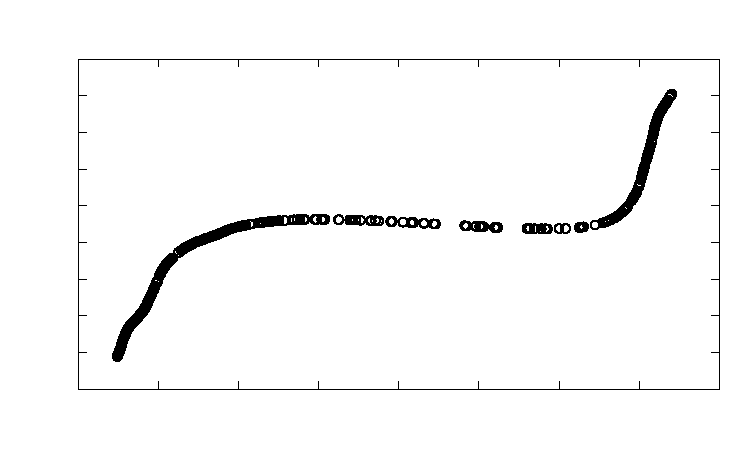
\includegraphics{GRAPH_color_graph4}}%
    \gplfronttext
  \end{picture}%
\endgroup

		% 			}\endgroup
		% 	\caption{Graph showing the colour-colour region for z=10-14. The colour window was defined as $f115w-f150w{\ge}14.439$ and $f150w-f200w{\le}14.815$\label{fig:col4}}
		% \end{figure}

	%subsection Results_for_Colour (end)

	\subsection{Interpretation of Colour Results}
	\label{sub:Interp_Colour}
		Constraining a colour window for observations turned out to be a challenging task. The filter 275w on James Webb didn't work properly in Hyperz; some magnitudes came out as 99.0 which is the default answer if there was an error; other magnitudes were above 100. As the source of this error could not be found, the range of redshift 14 to 15 was taken from the colour window results. The colour window results  shown in Figures ~\ref{fig:col1}, ~\ref{fig:col2}, ~\ref{fig:col3}  ~\ref{fig:col4} are much higher than expected results such as the colour windows in \cite{lorenzoni2013constraining}. Something must be wrong with the technique that was used to find the colours, however in defense of the results, the assumptions made as described in the sections above were reasonably fair for the timescale of the project. It's hard to say if there is one set of inputs or parameters that were the main source of error.  The shape of the distribtution of the galaxies is odd but seems to follow a pattern for each redshift range, which remains unexplained. The other peculiar characteristic of the diagrams is that all the galaxies appear on a mainly continous line, as opposed to being distributed in a certain area. Having done some basic tests, the cause of this appears to be due to setting the age of the galaxies at the same redshift to be the same; as soon as the age was randomised to some time between the formation redshift and the observed redshift, the galaxies were more spread out. However these galaxies appeared 'inside' the colour window, so this doesn't appear to have affected the determination of the colour windows. 

	%section Interpetation_of_colour_results (end)

%section Photometry_and_colour (end)




